\documentclass[tikz,border=6pt]{standalone}
\usepackage{amsmath,amssymb}
\usetikzlibrary{arrows.meta,patterns}
\begin{document}
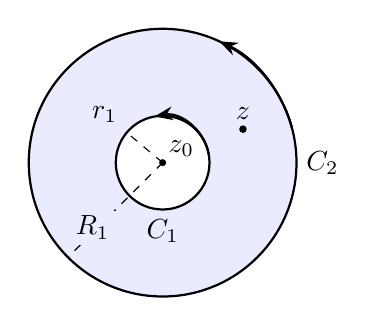
\begin{tikzpicture}[>=Stealth,scale=.85]
 \fill[blue!8,even odd rule] (0,0) circle (2) (0,0) circle (.7);
 \draw[thick] (0,0) circle (2);
 \draw[thick] (0,0) circle (.7);
 \draw[->,thick] (15:2) arc (15:65:2);
 \draw[->,thick] (10:.7) arc (10:100:.7);
 \fill (0,0) circle (1.5pt) node[above right,inner sep=2pt]{$z_0$};
 \fill (1.2,.5) circle (1.6pt) node[above]{$z$};
 \draw[dashed] (0,0)--(-135:2) node[midway,below left,fill=blue!8,inner sep=2pt]{$R_1$};
 \draw[dashed] (0,0)--(140:.7) node[above left]{$r_1$};
 \node[right] at (2,0) {$C_2$};
 \node[below] at (0,-.7) {$C_1$};
\end{tikzpicture}
\end{document}
